\documentclass{beamer}
\usepackage[utf8]{inputenc}
\usetheme{Madrid}
\usecolortheme{default}
\usepackage{amsmath,amssymb,amsfonts,amsthm}
\usepackage{txfonts}
\usepackage{tk\documentclass{beamer}
\usepackage[utf8]{inputenc}

\usetheme{Madrid}
\usecolortheme{default}
\usepackage{amsmath,amssymb,amsfonts,amsthm}
\usepackage{txfonts}
\usepackage{tkz-euclide}
\usepackage{listings}
\usepackage{adjustbox}
\usepackage{array}
\usepackage{tabularx}
\usepackage{gvv}
\usepackage{lmodern}
\usepackage{circuitikz}
\usepackage{tikz}
\usepackage{graphicx}

\setbeamertemplate{page number in head/foot}[totalframenumber]

\usepackage{tcolorbox}
\tcbuselibrary{minted,breakable,xparse,skins}

\definecolor{bg}{gray}{0.95}
\DeclareTCBListing{mintedbox}{O{}m!O{}}{%
breakable=true,
listing engine=minted,
listing only,
minted language=#2,
minted style=default,
minted options={%
linenos,
gobble=0,
breaklines=true,
breakafter=,,
fontsize=\small,
numbersep=8pt,
#1},
boxsep=0pt,
left skip=0pt,
right skip=0pt,
left=25pt,
right=0pt,
top=3pt,
bottom=3pt,
arc=5pt,
leftrule=0pt,
rightrule=0pt,
bottomrule=2pt,
toprule=2pt,
colback=bg,
colframe=orange!70,
enhanced,
overlay={%
\begin{tcbclipinterior}
\fill[orange!20!white] (frame.south west) rectangle ([xshift=20pt]frame.north west);
\end{tcbclipinterior}},
#3,
}
\lstset{
language=C,
basicstyle=\ttfamily\small,
keywordstyle=\color{blue},
stringstyle=\color{orange},
commentstyle=\color{green!60!black},
numbers=left,
numberstyle=\tiny\color{gray},
breaklines=true,
showstringspaces=false,
}

\title
{12.56}
\date{October 9, 2025}
\author
{EE25BTECH11043 - Nishid Khandagre}

\begin{document}

\frame{\titlepage}

\begin{frame}{Question}
The area enclosed between the curves $y^2 = 4x$ and $x^2 = 4y$ is 
\end{frame}

\begin{frame}{Theoretical Solution}
The equation of a parabola in Matrix form is
\begin{align}
\vec{x}^\top\vec{V}\vec{x} + 2\vec{u}^\top\vec{x} + f = 0
\end{align}
For $y^2 = 4x$:
\begin{align}
    \vec{V_1}=\begin{pmatrix}
        0 & 0\\
        0 & 1
    \end{pmatrix}
\end{align}
\begin{align}
    \vec{u_1}=-2\vec{e_1}=\myvec{-2\\0}\\
    f_1=0
\end{align}
\end{frame}

\begin{frame}{Theoretical Solution}
For $x^2 = 4y$:
\begin{align}
    \vec{V_2}=\begin{pmatrix}
        1 & 0\\
        0 & 0
    \end{pmatrix}
\end{align}
\begin{align}
    \vec{u_2}=-2\vec{e_2}=\myvec{0\\-2}\\
    f_2=0
\end{align}
The intersection of two conics with parameters $\vec{V_i}$, $\vec{u_i}$, $f_i$, $i=1,2$ is defined as 
\begin{align}
\vec{X}^{T}\,(\vec{V}_{1} + \mu \vec{V}_{2})\vec{X} + 2(\vec{u_1} + \mu \vec{u_2})^{T}\vec{X} \;+\; (f_{1} + \mu f_{2}) \;=\; 0 \label{eq:tem}
\end{align}
\end{frame}

\begin{frame}{Theoretical Solution}
\begin{align}
\implies \left|
\begin{array}{cc}
\mathbf{V}_1 + \mu \mathbf{V}_2 & \mathbf{u}_1 + \mu \mathbf{u}_2 \\[6pt]
(\mathbf{u}_1 + \mu \mathbf{u}_2)^{\mathrm{T}} & f_1 + \mu f_2
\end{array}
\right| = 0
\end{align}
\begin{align}
    \implies 
\left|
\begin{array}{ccc}
\mu & 0 & -2 \\[6pt]
0 & 1  & -2\mu \\[6pt]
-2 & -2\mu & 0
\end{array}
\right| = 0 
\end{align}
\end{frame}

\begin{frame}{Theoretical Solution}
\begin{align}
\implies \left|
\begin{array}{ccc}
\mu & 0 & -2 \\[6pt]
0 & 1  & -2\mu \\[6pt]
-2 & -2\mu & 0
\end{array}
\right| &\xleftrightarrow{R_3 \leftrightarrow R_3 + \frac{2}{\mu}\times R_1} \left|
\begin{array}{ccc}
\mu & 0 & -2 \\[6pt]
0 & 1  & -2\mu \\[6pt]
0 & -2\mu & -\frac{4}{\mu}
\end{array}
\right|\\
&\xleftrightarrow{R_3 \leftrightarrow R_3 + 2\mu \times R_2} \left|
\begin{array}{ccc}
\mu & 0 & -2 \\[6pt]
0 & 1  & -2\mu \\[6pt]
0 & 0 & -(\frac{4}{\mu} +4 \mu ^2)
\end{array}
\right| =0
\end{align}
\end{frame}

\begin{frame}{Theoretical Solution}
\begin{align}
\implies -(4 + 4 \mu ^3)=0\\
\implies \mu=-1
\end{align}
Substituting the value of $\mu=-1$ in $\eqref{eq:tem}$ we get points of intersection as 
\begin{align}
    \vec{x_1}=\myvec{0\\0} \\
    \vec{x_2}=\myvec{4\\4}
\end{align}
\end{frame}

\begin{frame}{Theoretical Solution}
Area of the desired region is given by
\begin{align}
A &= \int_{0}^{4}\left(2\sqrt{x}-\frac{x^2}{4}\right)dx\\
A &= \left[\frac{4}{3}x^{3/2} - \frac{x^3}{12}\right]_{0}^{4}
\end{align}
\end{frame}

\begin{frame}{Theoretical Solution}
\begin{align}
A &= \left(\frac{4}{3}(4)^{3/2} - \frac{(4)^3}{12}\right) - \left(0 - 0\right)\\
A &= \left(\frac{4}{3}(8) - \frac{64}{12}\right)\\
A &= \left(\frac{32}{3} - \frac{16}{3}\right)\\
A &= \frac{16}{3}
\end{align}
Thus, the area enclosed between the curves is $\frac{16}{3}$.
\end{frame}

\begin{frame}[fragile]
\frametitle{C Code}
\begin{lstlisting}[language=C]
#include <math.h>

// Function to calculate the area between y^2 = 4x and x^2 = 4y
double calculateEnclosedArea() {
    // The intersection points are (0,0) and (4,4)
    // The upper curve is y = 2*sqrt(x)
    // The lower curve is y = x*x / 4
    // Integral of (2*sqrt(x) - x*x / 4) from 0 to 4
    // Integral of 2*x^(1/2) is 2 * (x^(3/2) / (3/2)) = (4/3)*x^(3/2)
    // Integral of x^2 / 4 is (1/4) * (x^3 / 3) = x^3 / 12
\end{lstlisting}
\end{frame}

\begin{frame}[fragile]
\frametitle{C Code}
\begin{lstlisting}[language=C]
    // Evaluate at x=4:
    double upper_at_4 = (4.0/3.0) * pow(4.0, 1.5); // (4/3) * 8 = 32/3
    double lower_at_4 = pow(4.0, 3.0) / 12.0;       // 64 / 12 = 16/3

    // Evaluate at x=0 (both are 0)

    return upper_at_4 - lower_at_4; // 32/3 - 16/3 = 16/3
}
\end{lstlisting}
\end{frame}

\begin{frame}[fragile]
\frametitle{Python Code (using C shared library)}
\begin{lstlisting}[language=Python]
import ctypes
import numpy as np
import matplotlib.pyplot as plt

lib_area = ctypes.CDLL("/Users/nishidkhandagre/matgeo/venv/bin/code19.so")

# Define the argument types and return type for the C function
lib_area.calculateEnclosedArea.argtypes = []
lib_area.calculateEnclosedArea.restype = ctypes.c_double

# Call the C function to get the enclosed area
area_result = lib_area.calculateEnclosedArea()

print(f"The area enclosed between the curves y^2 = 4x and x^2 = 4y is: {area_result:.4f}")
\end{lstlisting}
\end{frame}

\begin{frame}[fragile]
\frametitle{Python Code (using C shared library)}
\begin{lstlisting}[language=Python]
# Generate points for plotting the curves
x_parabola = np.linspace(0, 5, 400) 
x_other_curve = np.linspace(0, 5, 400) 

# Curve 1: y^2 = 4x  =>  y = +/- 2*sqrt(x)
y_upper_parabola = 2 * np.sqrt(x_parabola)
y_lower_parabola = -2 * np.sqrt(x_parabola)

# Curve 2: x^2 = 4y  =>  y = x^2 / 4
y_other_curve = x_other_curve**2 / 4

# Plotting
plt.figure(figsize=(8, 8))

# Plot y^2 = 4x as a complete parabola
plt.plot(x_parabola, y_upper_parabola, 'b-', label=r'$y^2 = 4x$') 
plt.plot(x_parabola, y_lower_parabola, 'b-') 
\end{lstlisting}
\end{frame}

\begin{frame}[fragile]
\frametitle{Python Code (using C shared library)}
\begin{lstlisting}[language=Python]
# Plot x^2 = 4y
plt.plot(x_other_curve, y_other_curve, 'r-', label=r'$x^2 = 4y$')

# Fill the enclosed area 
x_fill = np.linspace(0, 4, 100)
y_upper_fill = 2 * np.sqrt(x_fill) 
y_lower_fill = x_fill**2 / 4       
plt.fill_between(x_fill, y_lower_fill, y_upper_fill, color='lightgray', alpha=0.5, label='Enclosed Area')

# Intersection points
plt.scatter([0, 4], [0, 4], color='green', s=100, zorder=5, label='Intersection Points')
plt.annotate('(0,0)', (0, 0), textcoords="offset points", xytext=(5,5), ha='left')
plt.annotate('(4,4)', (4, 4), textcoords="offset points", xytext=(5,5), ha='left')
\end{lstlisting}
\end{frame}

\begin{frame}[fragile]
\frametitle{Python Code (using C shared library)}
\begin{lstlisting}[language=Python]
plt.gca().set_aspect('equal', adjustable='box')
plt.xlabel('X-axis')
plt.ylabel('Y-axis')
plt.title(f'Area Enclosed Between $y^2=4x$ and $x^2=4y$')
plt.grid(True)
plt.legend()
plt.ylim(-5, 5) 
plt.xlim(-0.5, 5.5) 
plt.show()
\end{lstlisting}
\end{frame}

\begin{frame}[fragile]
\frametitle{Python Code (Direct)}
\begin{lstlisting}[language=Python]
import numpy as np
import matplotlib.pyplot as plt

# Define the functions for the two curves
def curve1_y_positive(x):
    return 2 * np.sqrt(x)  

def curve1_y_negative(x):
    return -2 * np.sqrt(x) 

def curve2_y(x):
    return x**2 / 4  

# Define the range for x
x_parabola1 = np.linspace(0, 10, 400) 
x_parabola2 = np.linspace(-6, 6, 400) 
\end{lstlisting}
\end{frame}

\begin{frame}[fragile]
\frametitle{Python Code (Direct)}
\begin{lstlisting}[language=Python]
# Calculate y values for each curve
y1_positive = curve1_y_positive(x_parabola1)
y1_negative = curve1_y_negative(x_parabola1)
y2 = curve2_y(x_parabola2)

# Plotting the curves
plt.figure(figsize=(9, 7))

# Plot y^2 = 4x (full parabola)
plt.plot(x_parabola1, y1_positive, color='blue', label='$y^2 = 4x$ (upper part)')
plt.plot(x_parabola1, y1_negative, color='blue', linestyle='--', label='$y^2 = 4x$ (lower part)')

# Plot x^2 = 4y (full parabola)
plt.plot(x_parabola2, y2, color='green', label='$x^2 = 4y$')
\end{lstlisting}
\end{frame}

\begin{frame}[fragile]
\frametitle{Python Code (Direct)}
\begin{lstlisting}[language=Python]
# Shade the enclosed area between (0,0) and (4,4)
x_fill = np.linspace(0, 4, 100)
y_upper_bound = 2 * np.sqrt(x_fill)
y_lower_bound = x_fill**2 / 4
plt.fill_between(x_fill, y_upper_bound, y_lower_bound, color='lightgray', alpha=0.5, label='Enclosed Area')

# Add intersection points
intersection_x = [0, 4]
intersection_y = [0, 4]
plt.scatter(intersection_x, intersection_y, color='red', zorder=5, label='Intersection Points')
plt.text(0.1, 0.1, '(0,0)', fontsize=10, verticalalignment='bottom')
plt.text(4.2, 4.2, '(4,4)', fontsize=10, verticalalignment='bottom')
\end{lstlisting}
\end{frame}

\begin{frame}[fragile]
\frametitle{Python Code (Direct)}
\begin{lstlisting}[language=Python]
# Add labels and title
plt.xlabel('$x$')
plt.ylabel('$y$')
plt.title('Full Parabolas and Enclosed Area')
plt.legend()
plt.grid(True)
plt.axhline(0, color='black',linewidth=0.5)
plt.axvline(0, color='black',linewidth=0.5)
plt.xlim(-2, 11) 
plt.ylim(-7, 7)  
plt.gca().set_aspect('equal', adjustable='box')

# Show the plot
plt.savefig("full_parabolas_enclosed_area.png")
plt.show()

print("Figure saved as full_parabolas_enclosed_area.png")
print(f"The calculated enclosed area is: {16/3:.2f} square units")
\end{lstlisting}
\end{frame}

\begin{frame}{Plot by Python using shared output from C}
\begin{figure}[H]
\centering
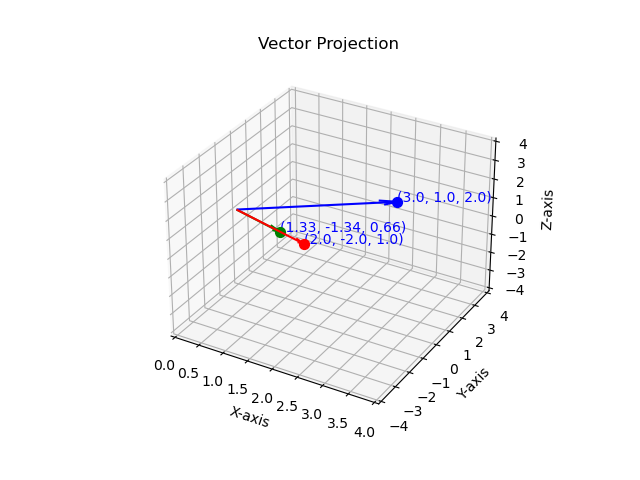
\includegraphics[width=0.8\columnwidth]{../figs/fig1.png}
\caption{}
\label{fig:1}
\end{figure}
\end{frame}

\begin{frame}{Plot by Python only}
\begin{figure}[H]
\centering
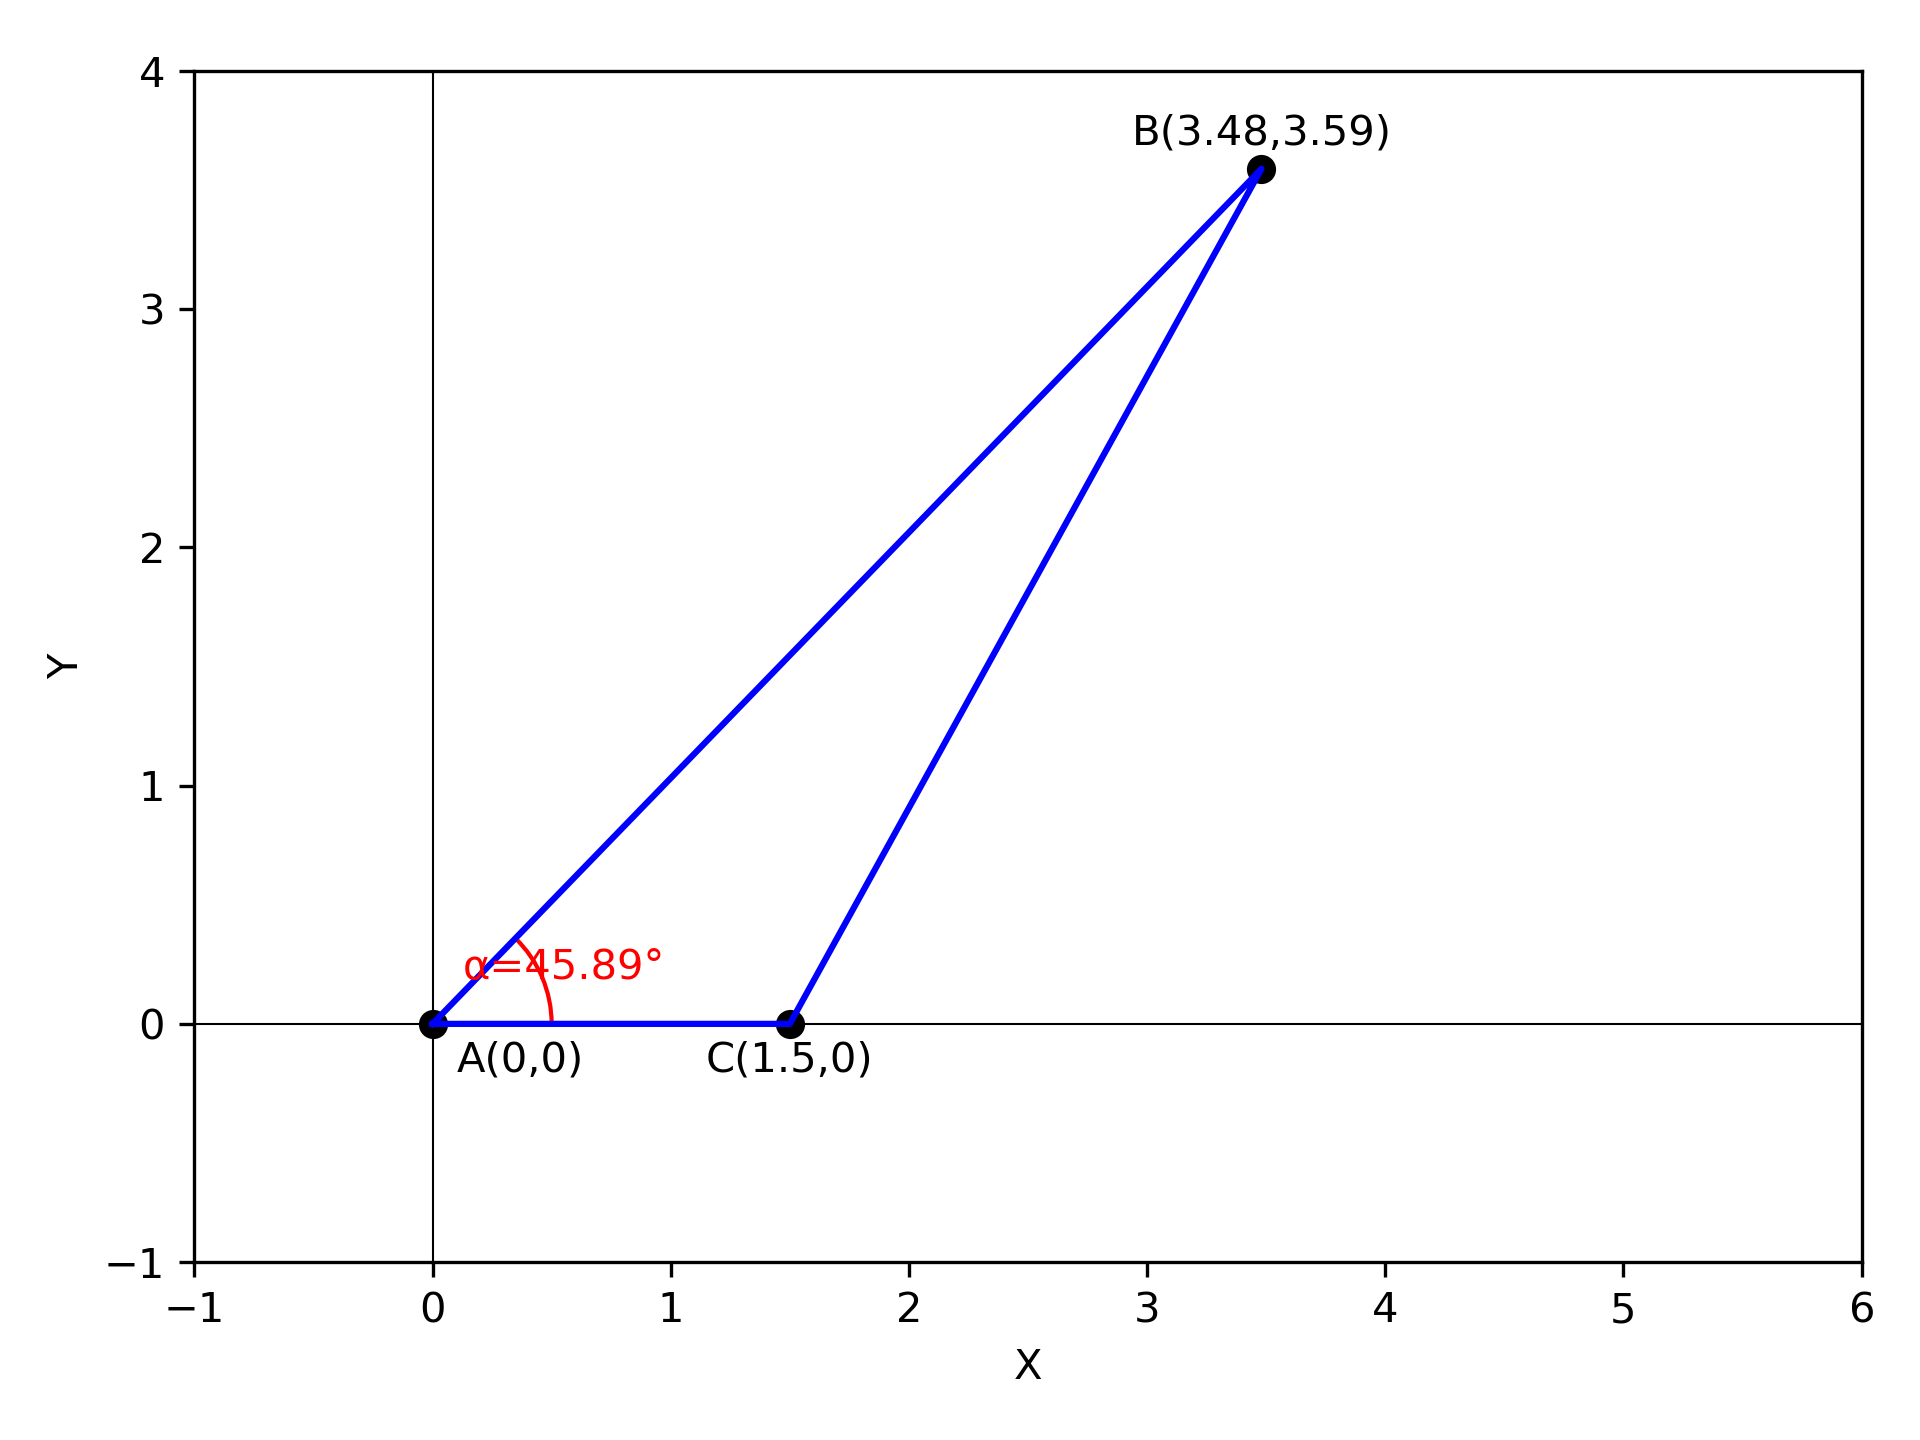
\includegraphics[width=0.8\columnwidth]{../figs/fig2.png}
\caption{}
\label{fig:2}
\end{figure}
\end{frame}

\end{document}
z-euclide}
\usepackage{listings}
\usepackage{adjustbox}
\usepackage{array}
\usepackage{tabularx}
\usepackage{gvv}
\usepackage{lmodern}
\usepackage{circuitikz}
\usepackage{tikz}
\usepackage{graphicx}

\setbeamertemplate{page number in head/foot}[totalframenumber]

\usepackage{tcolorbox}
\tcbuselibrary{minted,breakable,xparse,skins}



\definecolor{bg}{gray}{0.95}
\DeclareTCBListing{mintedbox}{O{}m!O{}}{%
  breakable=true,
  listing engine=minted,
  listing only,
  minted language=#2,
  minted style=default,
  minted options={%
    linenos,
    gobble=0,
    breaklines=true,
    breakafter=,,
    fontsize=\small,
    numbersep=8pt,
    #1},
  boxsep=0pt,
  left skip=0pt,
  right skip=0pt,
  left=25pt,
  right=0pt,
  top=3pt,
  bottom=3pt,
  arc=5pt,
  leftrule=0pt,
  rightrule=0pt,
  bottomrule=2pt,
  toprule=2pt,
  colback=bg,
  colframe=orange!70,
  enhanced,
  overlay={%
    \begin{tcbclipinterior}
    \fill[orange!20!white] (frame.south west) rectangle ([xshift=20pt]frame.north west);
    \end{tcbclipinterior}},
  #3,
}
\lstset{
    language=C,
    basicstyle=\ttfamily\small,
    keywordstyle=\color{blue},
    stringstyle=\color{orange},
    commentstyle=\color{green!60!black},
    numbers=left,
    numberstyle=\tiny\color{gray},
    breaklines=true,
    showstringspaces=false,
}

%\numberwithin{equation}{section}

\title{Matgeo-q.5.13.12}
\author{AI25BTECH11036-SNEHAMRUDULA}

\date{\today} 
\begin{document}
\begin{frame}
\titlepage
\end{frame}

\section*{Outline}
\begin{frame}{question}
Find the set of all values of $\lambda$ for which the system
\[
\begin{aligned}
2x_1-2x_2+x_3 &= \lambda x_1,\\
2x_1-3x_2+2x_3 &= \lambda x_2,\\
- x_1+2x_2 &= \lambda x_3
\end{aligned}
\]
has a non-trivial solution. Which of the following is true?
 \item  \textbf{A)}contains two elements
\item   \textbf{B)} contains more than two elements
 \item  \textbf{C)}is an empty set
\item   \textbf{D)}is a singlet
  \end{frame}
\begin{frame}{solution}
Bring all terms to one side:

\[
\begin{aligned}
(2 - \lambda)x_1 - 2x_2 + x_3 &= 0 \\
2x_1 + (-3 - \lambda)x_2 + 2x_3 &= 0 \\
-x_1 + 2x_2 - \lambda x_3 &= 0
\end{aligned}
\]


\[
\myvec{
2 - \lambda & -2 & 1 \\
2 & -3 - \lambda & 2 \\
-1 & 2 & -\lambda
}
\vec{x}
= \vec{0}
\quad \text{where} \quad
\vec{x} = \myvec{x_1 \\ x_2 \\ x_3},\quad \vec{0} = \myvec{0 \\ 0 \\ 0}
\]
\[
\text{rank}(\text{Coefficient Matrix}) < 3
\]
\[
\text{rank}\left(
\myvec{
2 - \lambda & -2 & 1 \\
2 & -3 - \lambda & 2 \\
-1 & 2 & -\lambda
}
\right) = 2
\]
So, the system has a non-trivial solution for exactly two values of \( \lambda \).

\[
\boxed{\text{Correct answer: (a) contains two elements}}
\]
\end{frame}
    \begin{frame}{Graphical Representation}
   \begin{figure}[h!]
\centering
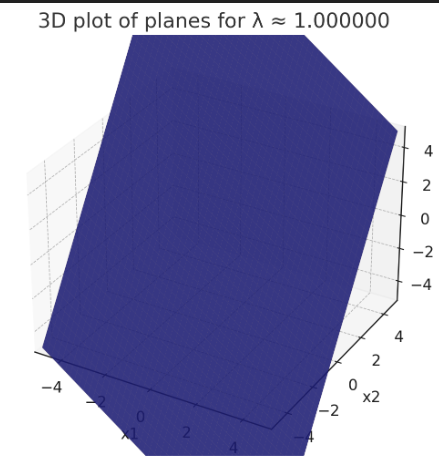
\includegraphics[width=0.6\linewidth]{5.13.12fig.png}
\end{figure}
\end{frame}
   \begin{figure}[h!]
\centering
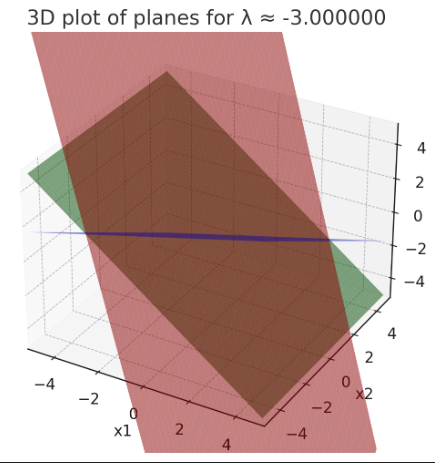
\includegraphics[width=0.6\linewidth]{5.13.12fig(1).png}
\end{figure}
\end{frame}
\end{document}